%
%   N K Y M
%    A A A A
%

%   this file is "nkym.tex"

\documentclass[10pt,b5paper,papersize,dvipdfmx]{jsbook}

\usepackage{vuccaken}
\usepackage{vuccaken2019}

\begin{document} % 以下本文

% - - - - - - - - - - - - - - - - - - - - - - - - %
\kaishititle%
  {こてんりきがくではない}% title
  {物理科学科4回生}% 所属
  {中山 敦貴}% name
% - - - - - - - - - - - - - - - - - - - - - - - - %

% \setcounter{tocdepth}{2} % 目次にどこまで表示するか
% \tableofcontents % 目次出力
% \clearpage % 改ページ

first commit!!

%
\section*{はじめに}
とりあえず、内容としましては、古典力学で仮定されていた局所実在論では説明できないようなことが量子の世界では起こっているという話をします。
具体的には、局所実在論であれば必ず成立するベルの不等式が、エンタングルメントという量子論特有の性質を持った系では破れることがあるということを示します。\par
章立ては大きくは以下のような感じだと思います。


%
\section{局所実在論}

%
\section{ベルの不等式}

%
\section{量子エンタングルメント}

%
\section{解釈?}


% \begin{figure}[htbp]
%   \centering
%   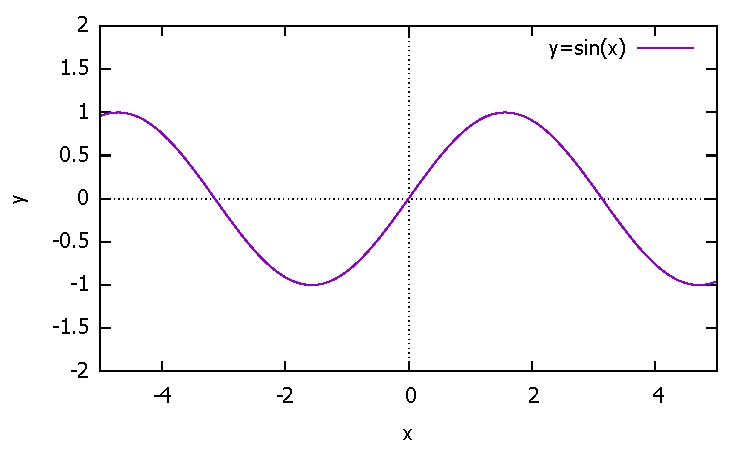
\includegraphics[width=10cm]{temp/fig-sin.pdf}
%   \caption{$y=\sin x$のグラフ。gnuplotで作成した。}
%   \label{fig:sin}
% \end{figure}

\clearpage

%% 参考文献
\begin{sanko}
  \begin{enumerate}
    \item 清水明、「新版 量子論の基礎」、サイエンス社、2004年。
    \item 清水明、スライド「EPRパラドックスからベルの不等式へ」\\
      \url{http://as2.c.u-tokyo.ac.jp/lecture_note/kstext04_ohp.pdf}
    \item J.J.サクライ、「現代の量子力学(上)」、吉岡書店。
    \item 森田邦久、「アインシュタイン vs. 量子力学」、化学同人。
    \item 森田邦久、「量子力学の哲学」、講談社現代新書。
    \item 荒船次郎 他、「現代物理学の歴史 I」、朝倉書店。
  \end{enumerate}
\end{sanko}


\end{document}
%
% EOF
%